\documentclass[1p]{elsarticle}        	% 5p gives 2 columns pr page, 1p gives 1.
\journal{Ingve Simonsen}
\usepackage{graphicx}
\usepackage{amsmath,amssymb}
\usepackage{booktabs}			% Nicer tables etc.
\usepackage{hyperref}
\usepackage[]{todonotes}

%\usepackage[section]{below}        %Confine figures to their sections

%%%%%%%%%%%%%%%%%%%%%%%%%%%%%%%%%%%%%%%%%%%%%%%%%%%%%%%%%%%%%%%%%%%%%%%%%
\begin{document}
\begin{frontmatter}
\title{Title}
\author{Paul Thrane}
%\address[fysikk]{Institutt for fysikk, Norges Teknisk-Naturvitenskapelige Universitet, N-7491 Trondheim, Norway.}
\begin{abstract}
A catchy abstract.

\end{abstract}
\end{frontmatter}
%%%%%%%%%%%%%%%%%%%%%%%%%%%%%%%%%%%%%%%%%%%%%%%%%%%%%%%%%%%%%%%%%%%%%%%%%
\section{Main Body}
An intriguing introduction, followed by something cool. \nocite{*}

\begin{figure}
	\centering
	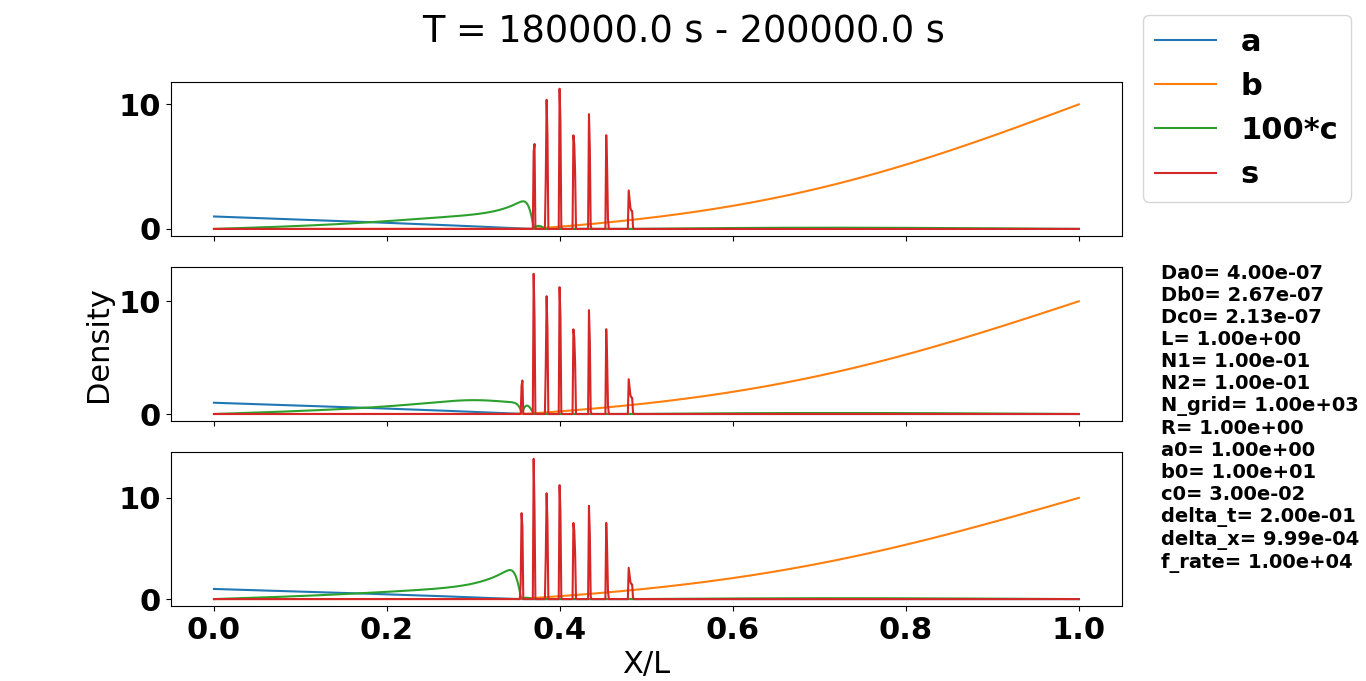
\includegraphics[width=\linewidth]{../figures/standard_settings_time.png}
	\caption{Coordinates.}
	\label{fig:coords}
\end{figure}

\begin{figure}
	\centering
	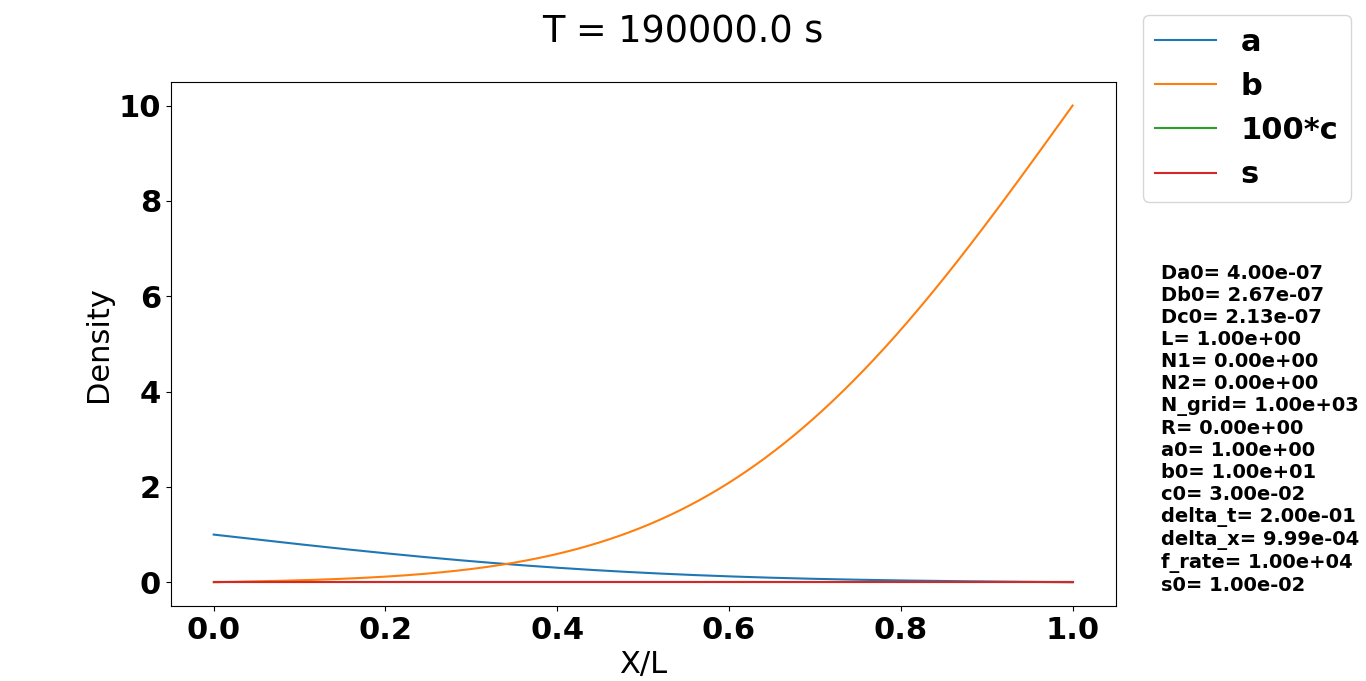
\includegraphics[width=\linewidth]{../figures/R0.png}
	\caption{Coordinates.}
	\label{fig:coords}
\end{figure}

\begin{figure}
	\centering
	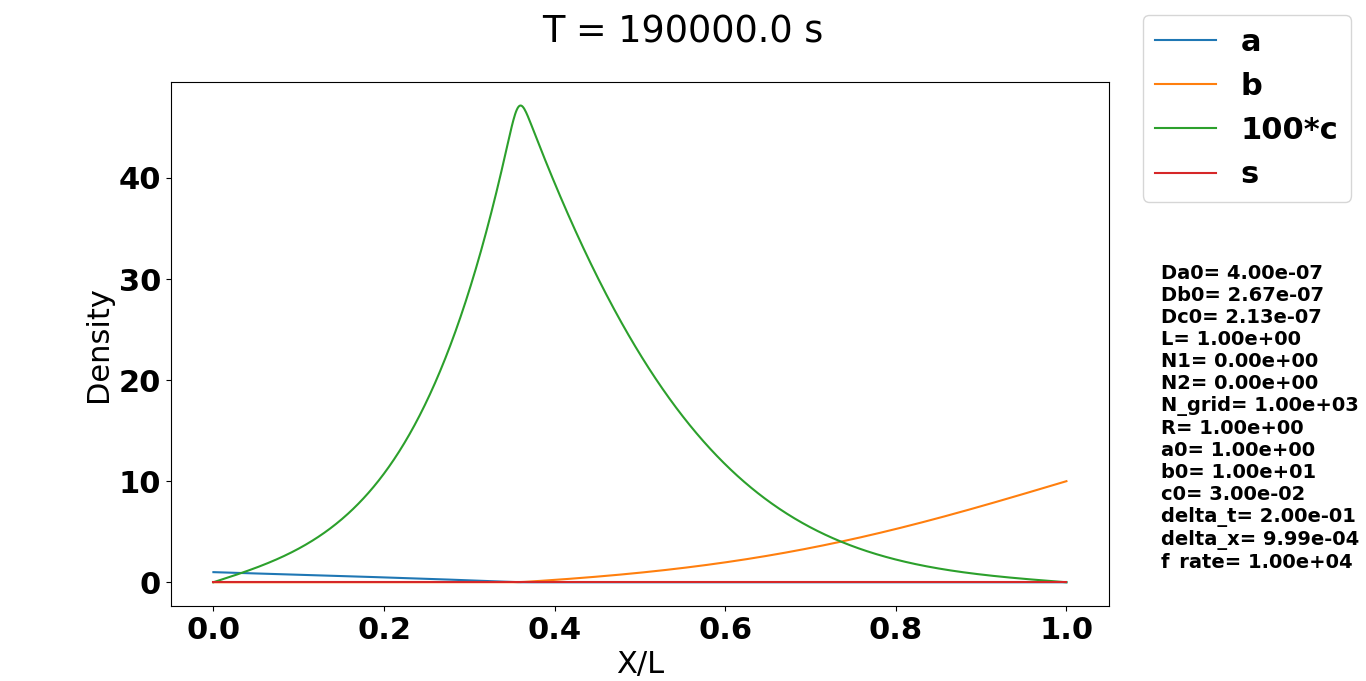
\includegraphics[width=\linewidth]{../figures/N0.png}
	\caption{Coordinates.}
	\label{fig:coords}
\end{figure}

\begin{figure}
	\centering
	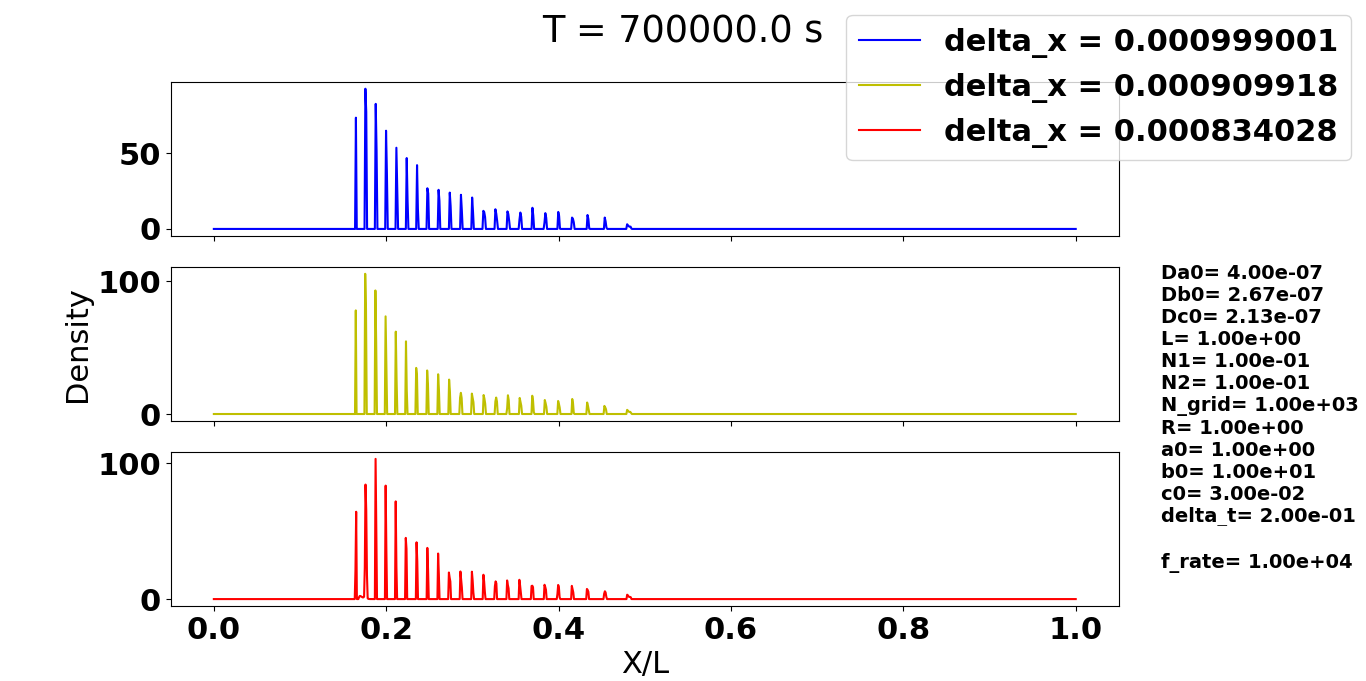
\includegraphics[width=\linewidth]{../figures/deltaX.png}
	\caption{Coordinates.}
	\label{fig:coords}
\end{figure}

\begin{figure}
	\centering
	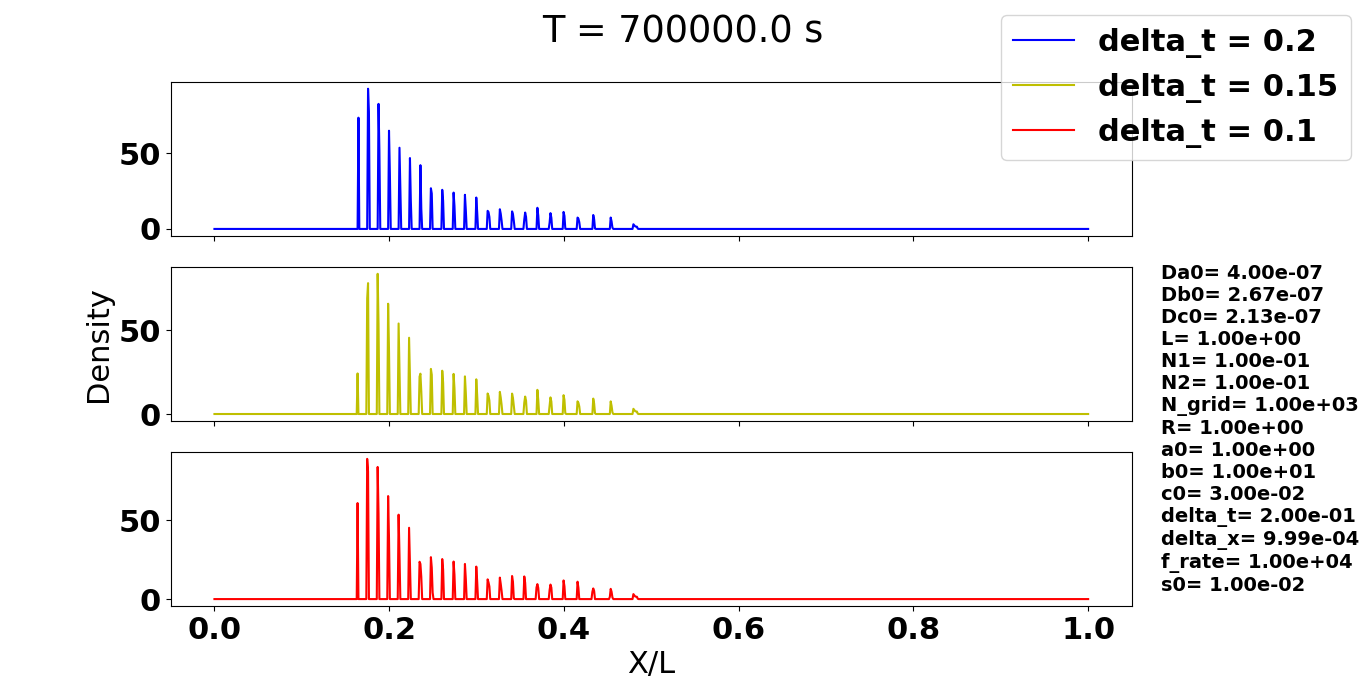
\includegraphics[width=\linewidth]{../figures/deltaT.png}
	\caption{Coordinates.}
	\label{fig:coords}
\end{figure}

\begin{figure}
	\centering
	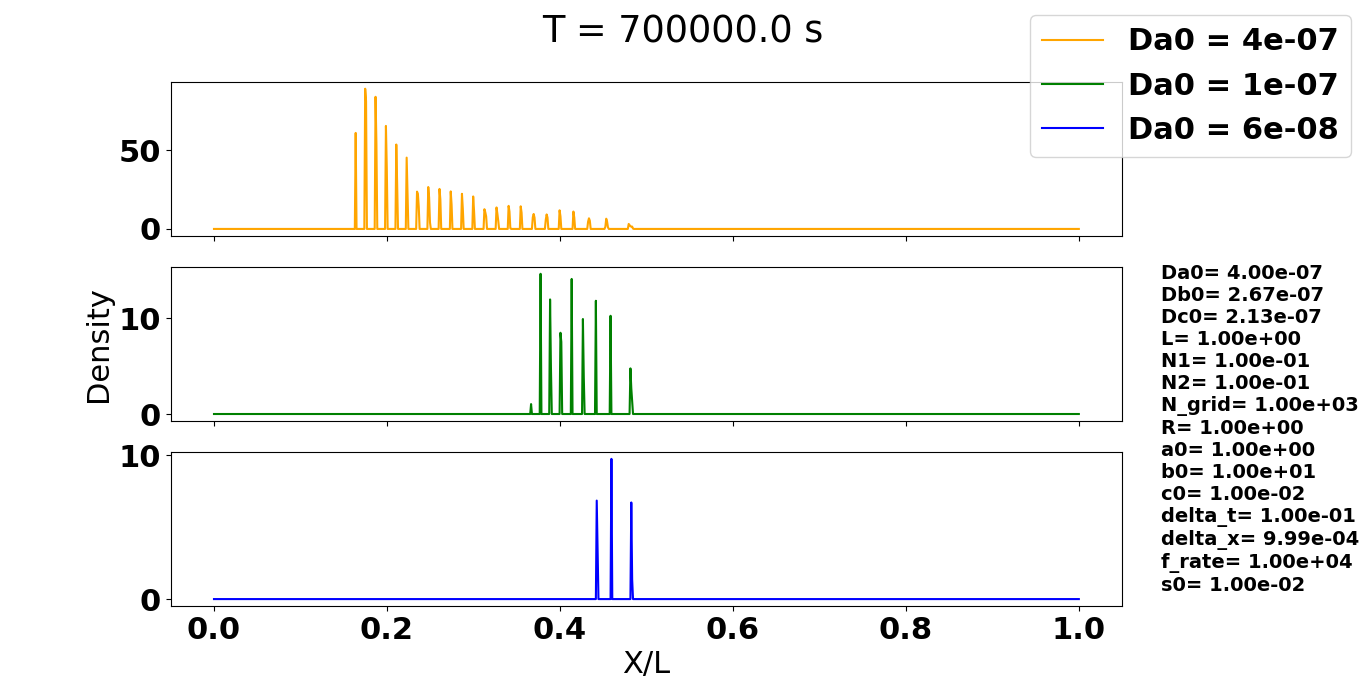
\includegraphics[width=\linewidth]{../figures/Da0_same_ratio.png}
	\caption{Coordinates.}
	\label{fig:coords}
\end{figure}

\begin{figure}
	\centering
	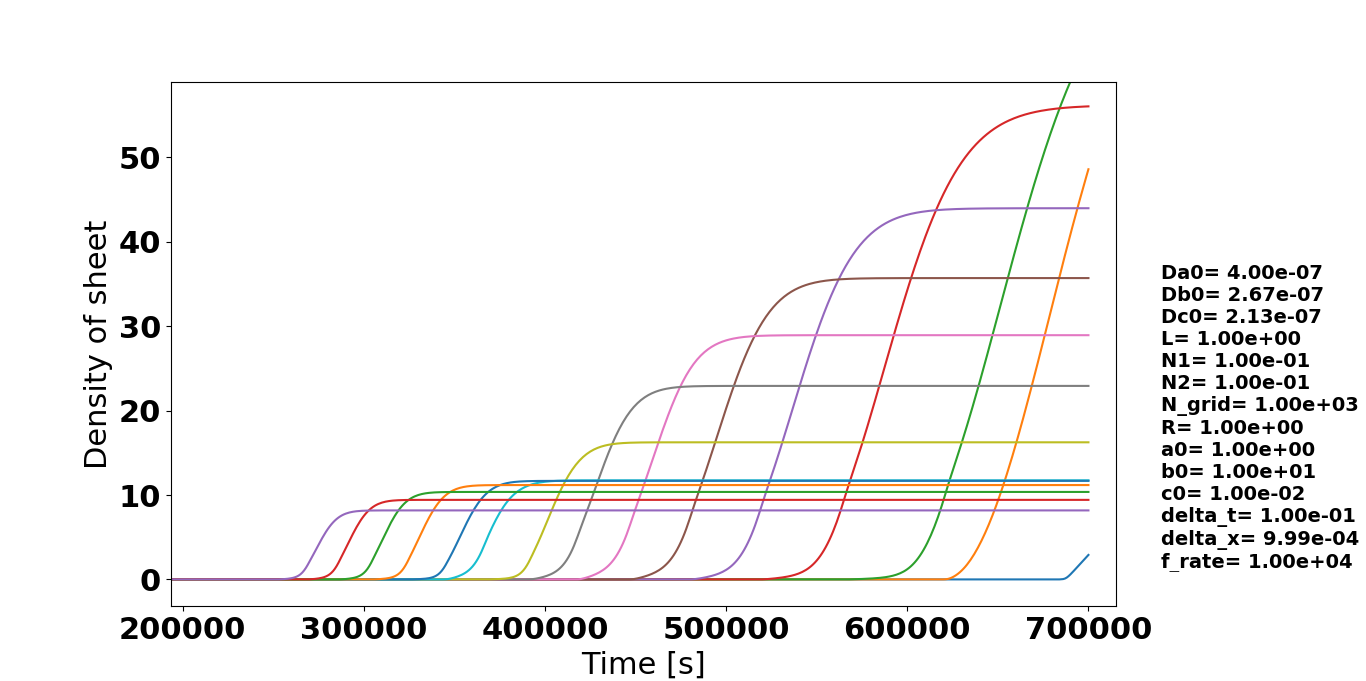
\includegraphics[width=\linewidth]{../figures/peak_growth.png}
	\caption{Coordinates.}
	\label{fig:coords}
\end{figure}

\begin{figure}
	\centering
	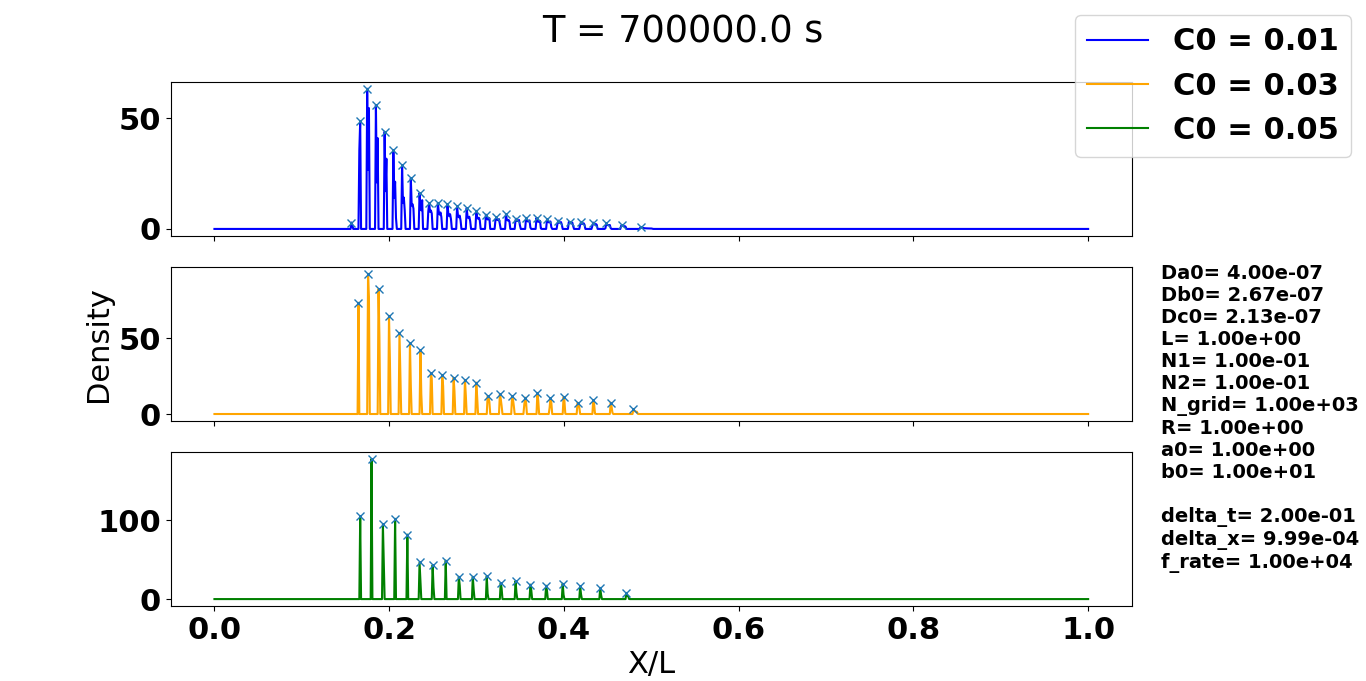
\includegraphics[width=\linewidth]{../figures/deltaC0_s.png}
	\caption{Coordinates.}
	\label{fig:coords}
\end{figure}

\begin{figure}
	\centering
	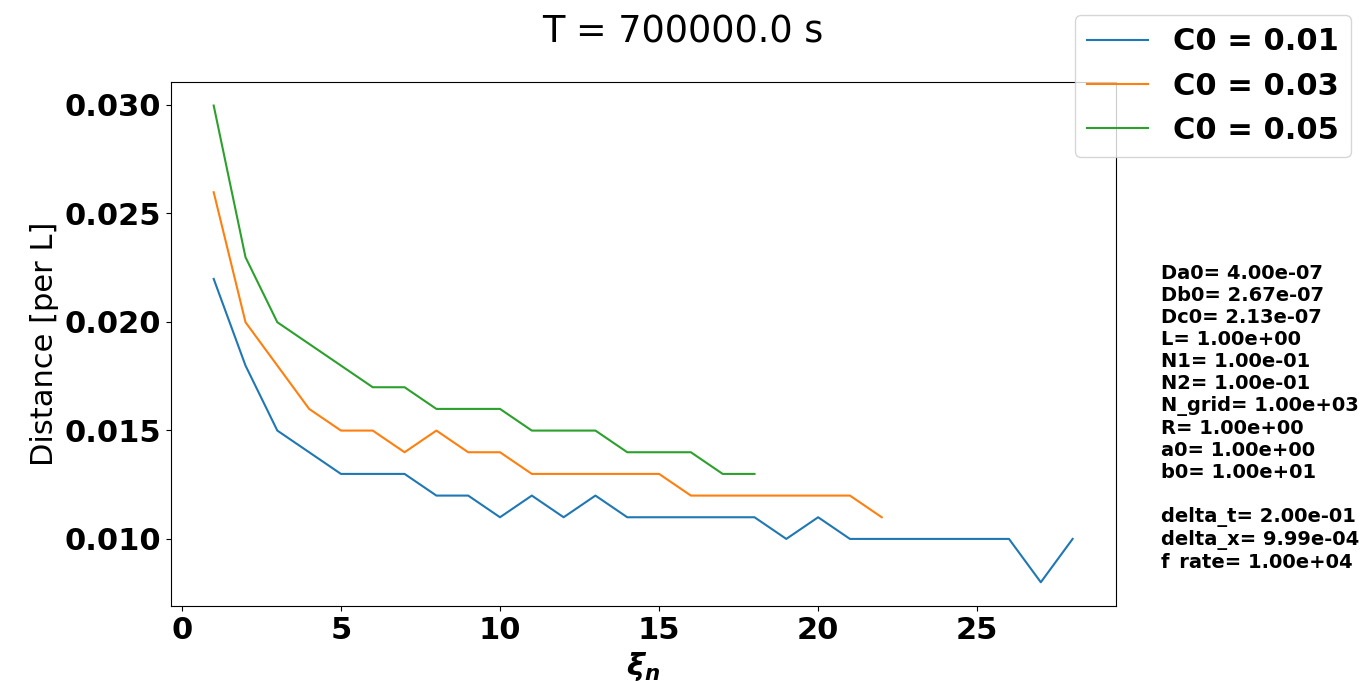
\includegraphics[width=\linewidth]{../figures/deltaC0_x.png}
	\caption{Coordinates.}
	\label{fig:coords}
\end{figure}

\begin{figure}
	\centering
	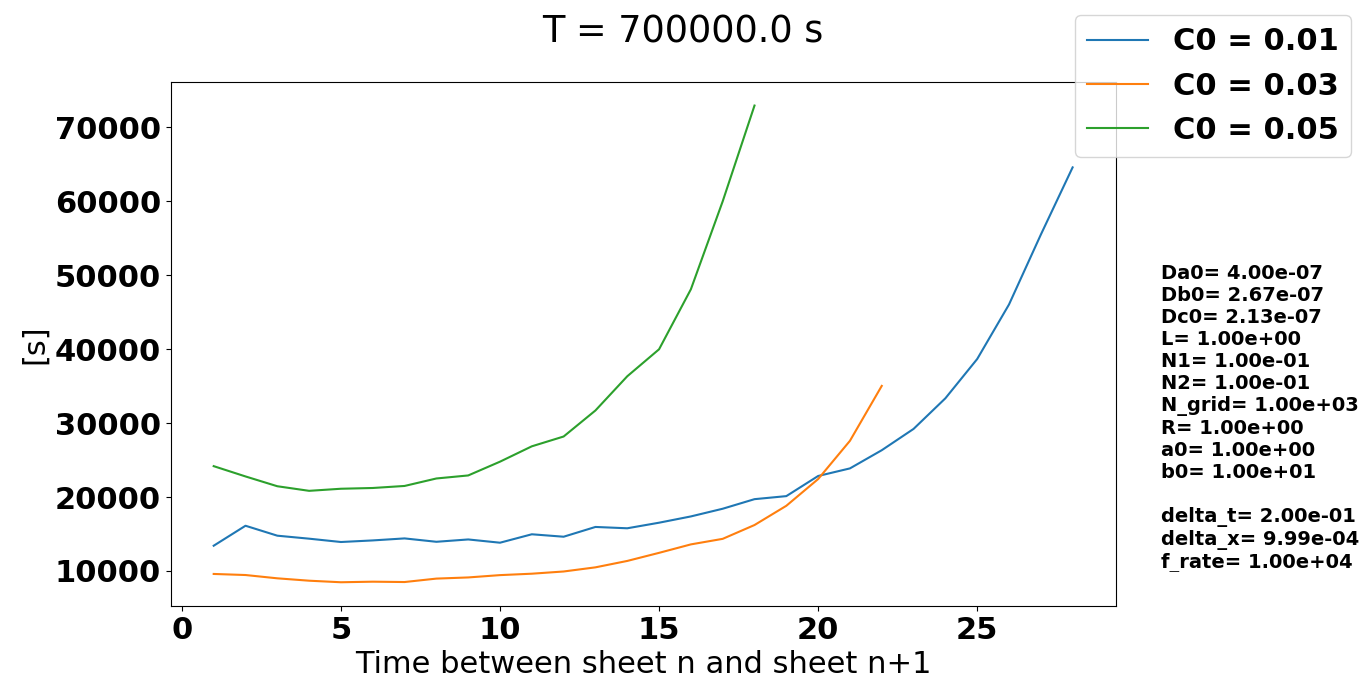
\includegraphics[width=\linewidth]{../figures/deltaC0_t.png}
	\caption{Coordinates.}
	\label{fig:coords}
\end{figure}

\begin{figure}
	\centering
	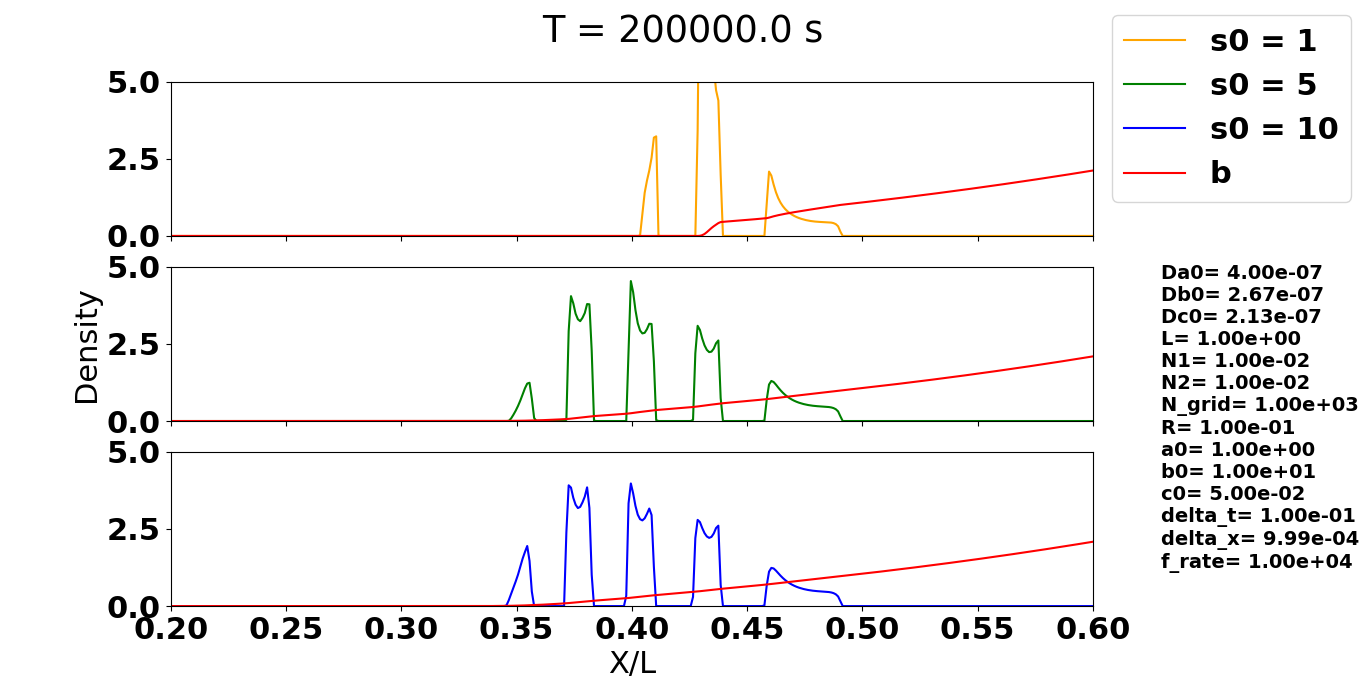
\includegraphics[width=\linewidth]{../figures/s0_1-10.png}
	\caption{Coordinates.}
	\label{fig:coords}
\end{figure}

\begin{figure}
	\centering
	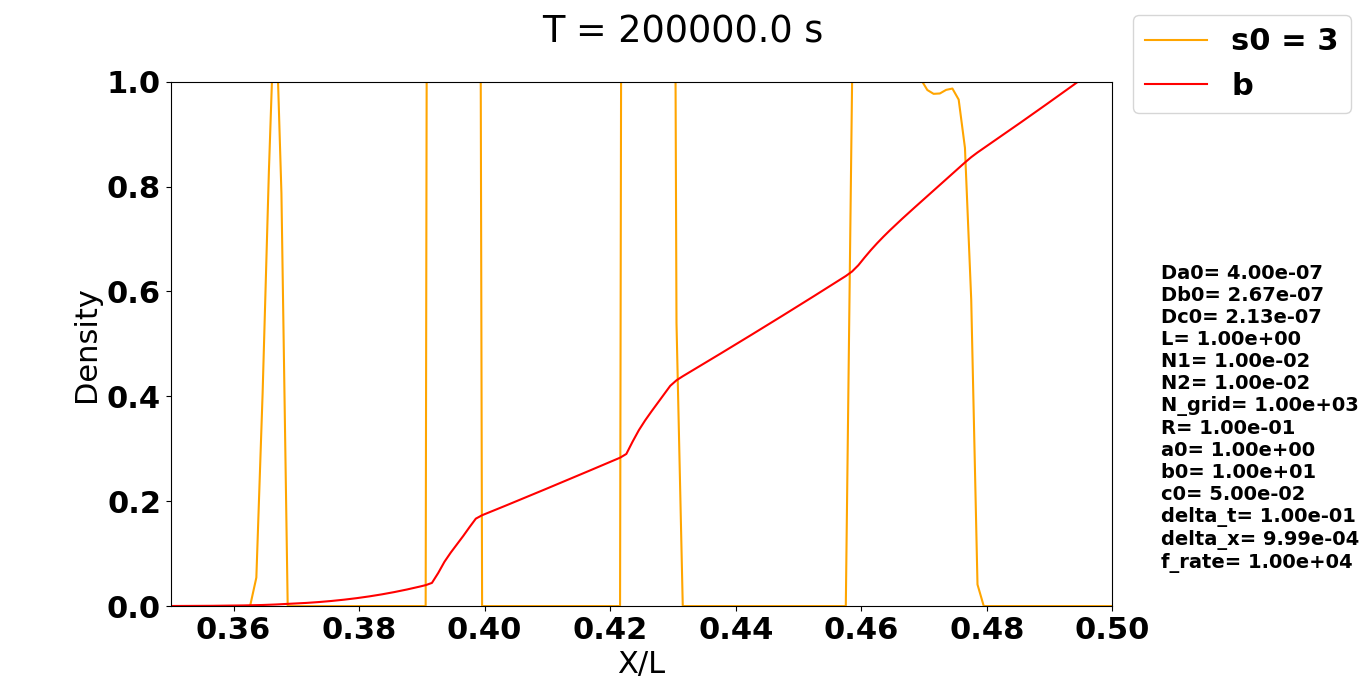
\includegraphics[width=\linewidth]{../figures/s0_3.png}
	\caption{Coordinates.}
	\label{fig:coords}
\end{figure}

\begin{figure}
	\centering
	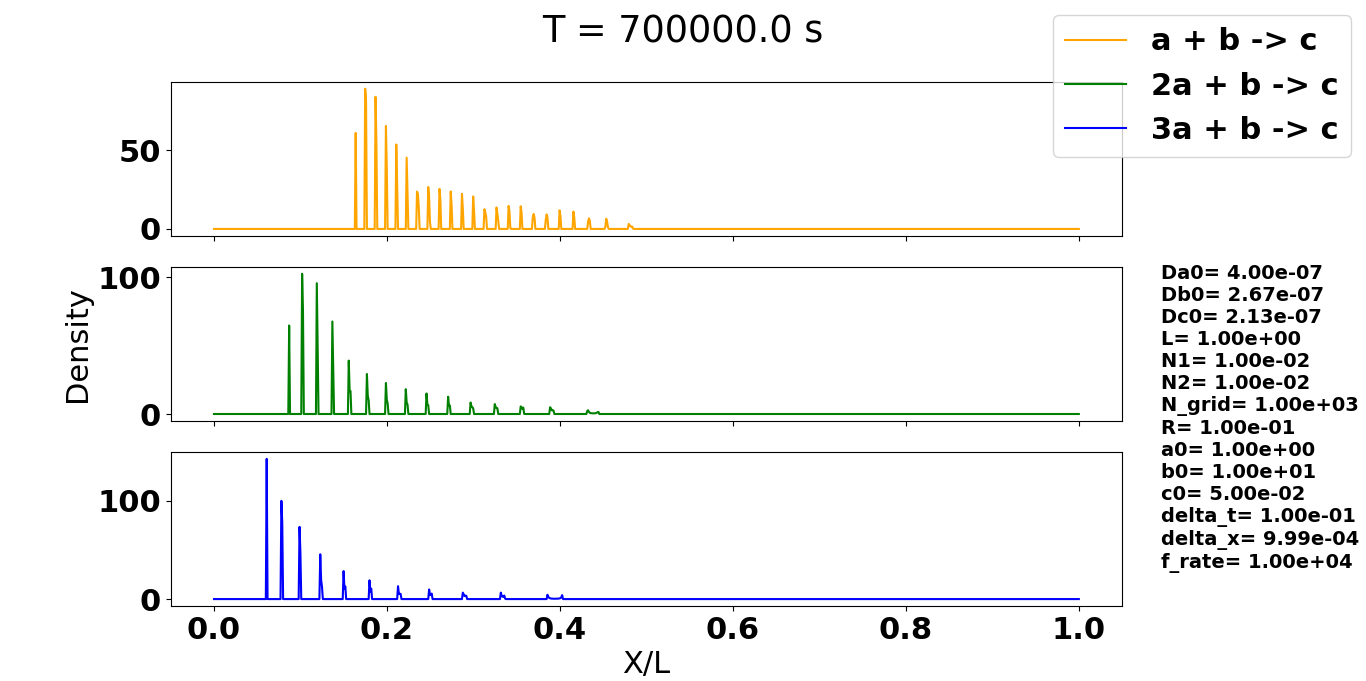
\includegraphics[width=\linewidth]{../figures/2a_s.png}
	\caption{Coordinates.}
	\label{fig:coords}
\end{figure}






\section*{References}
\bibliographystyle{elsart-num}
\bibliography{bibl}  

\end{document}